

\chapter{Sistema de Filtragem de Eventos do ATLAS}
\label{cap:trigger}
\glsresetall


A maioria das reações de interresse ocorrem com frequência bastante reduzida, uma vez que esses
eventos são bastante raros. Por outro lado, jatos hadrônicos possuem uma frequência da ordem de centenas de $k$Hz, sendo necessários
descartá-los da cadeia de processamento. Além da taxa de colisões, a granularidade dos detectores 
envolvidos na aquisição dos eventos colabora, de forma crucial, com o volume de informação gerado.

À cada colisão, aproximadamente 1,5 MBytes de informação serão 
produzidos.  Ao multiplicar-se este valor pela taxa de colisões, obtém-se um volume de informação da ordem de 60 TBytes por segundo. 
Adicionalmente, canais físicos de interesse ocorrem com um período que varia de algumas horas a até dias de operação. 
Consequentemente, um sistema de filtragem online torna-se indispensável para o experimento. O sistema de filtragem deverá identificar os 
padrões de decaimento do \textit{Higgs}, e demais eventos de interesse, para poder localiza-los na massa de eventos com física ordinária (interações 
que produzem canais físicos já conhecidos e que, portanto, significam ruído de fundo para o experimento).

Nos sistemas de filtragem  \textit{online}, utiliza-se um sistema hierárquico de análise, onde os níveis superiores validam a decisão dos níveis inferiores. 
Tipicamente, a hierarquia de análise de um sistema de filtragem \textit{online} é desenvolvida de forma que os níveis mais baixos apliquem cortes baseados em critérios 
de análise mais simples, enquanto que níveis mais elevados implementam critérios de seleção mais complexos, uma vez que dispõem de um tempo maior para 
análise de cada evento. Entretanto, como os níveis mais altos operam sobre um subconjunto de eventos que não foram rejeitados pelos níveis inferiores, estes 
sistemas de filtragem hierárquicos não podem desfazer a rejeição aplicada por um nível mais baixo. Os tópicos a seguir irão abordar o sistema de nível 1 e 
o Trigger de alto nível somente para o canal e/$\gamma$.

\subsection{Primeiro Nível de Trigger}

O primeiro nível de filtragem (L1) realiza a seleção inicial, baseando-se na informação obtida com granularidade reduzida de um subconjunto dos detectores.
Devido ao alto número de canais dos detectores de traço e ao alto custo computacional dos algoritmos nesses detectores, optou-se por utiliza somente a 
informação dos calorímetros e dos detectores rápidos de múons para compor a informação do primeiro nível de Trigger.  A granularidade neste nível não é 
plena, uma vez que o tempo para a tomada de decisão neste nível é da ordem de microsegundos. Uma outra característica deste nível é que todo ele é implementado 
em $hardware$ programáves como \gls{fpga}, o que garante uma maior flexibilidade aos projetos e permite a implementação de algoritmos mais complexos 
utilizando-se linguagens de alto nível dentro de um ambiente de circuitos integrados.

A redução da quantidade de informação neste nível é crucial devido aos seus requisitos de latência. Assim, agrupam-se as células dos calorímetros 
(eletromagnético e hadrônico) em um conjunto contendo 6 células. As células de cada conjunto são analogicamente somadas, produzindo um único
sinal e este é comparado com um limiar de corte de energia pré-definido. Consequentemente, este primeiro nível só descarta eventos com características 
bastante distintas dos canais de interesse. Por exemplo, um par de eventos eletromagnéticos isolados com $E_{t} > 20GeV$ são importantes para o estudo
do canal $H \rightarrow ZZ \rightarrow 4ee$ (bóson de Higgs decaindo em 2$Z$, cada um decaindo em 2 elétrons).    

A detecção de elétrons no L1 é feita utilizando algoritmos velozes, dado o pequeno tempo de latência existente neste nível. Consequentemente, a seleção
é feita através de cortes simples, utilizando informações triviais obtidas a partir da leitura de células do calorímetro. Estas informações são obtidas analisando-se
a energia transversa do evento e o perfil lateral e longitudinal do chuveiro produzido.  O algoritmo de filtragem para elétrons está ilustrado na Figura~\ref{fig:sliding_window_l1}. Este algoritmo é baseado em uma janela contendo $4\times4$ torres de \textit{Trigger}\footnote{Cada torre de \textit{Trigger} possui granularidade de $0,1\times0,1$ em $\eta\times\phi$ e é produzida pela soma analógica das células do calorímetro.} em $\eta\times\phi$, tanto para o calorímetro eletromagnético como para o hadrônico. A janela percorre todo o calorímetro ($|\eta|$ < 2,5) em passos de uma torre, tanto em $\eta$ quanto em $\phi$. O L1 seleciona o evento como um possível candidato a $e/\gamma$ quando os seguintes critérios forem aprovados:

\begin{figure}[h!t]
\centering
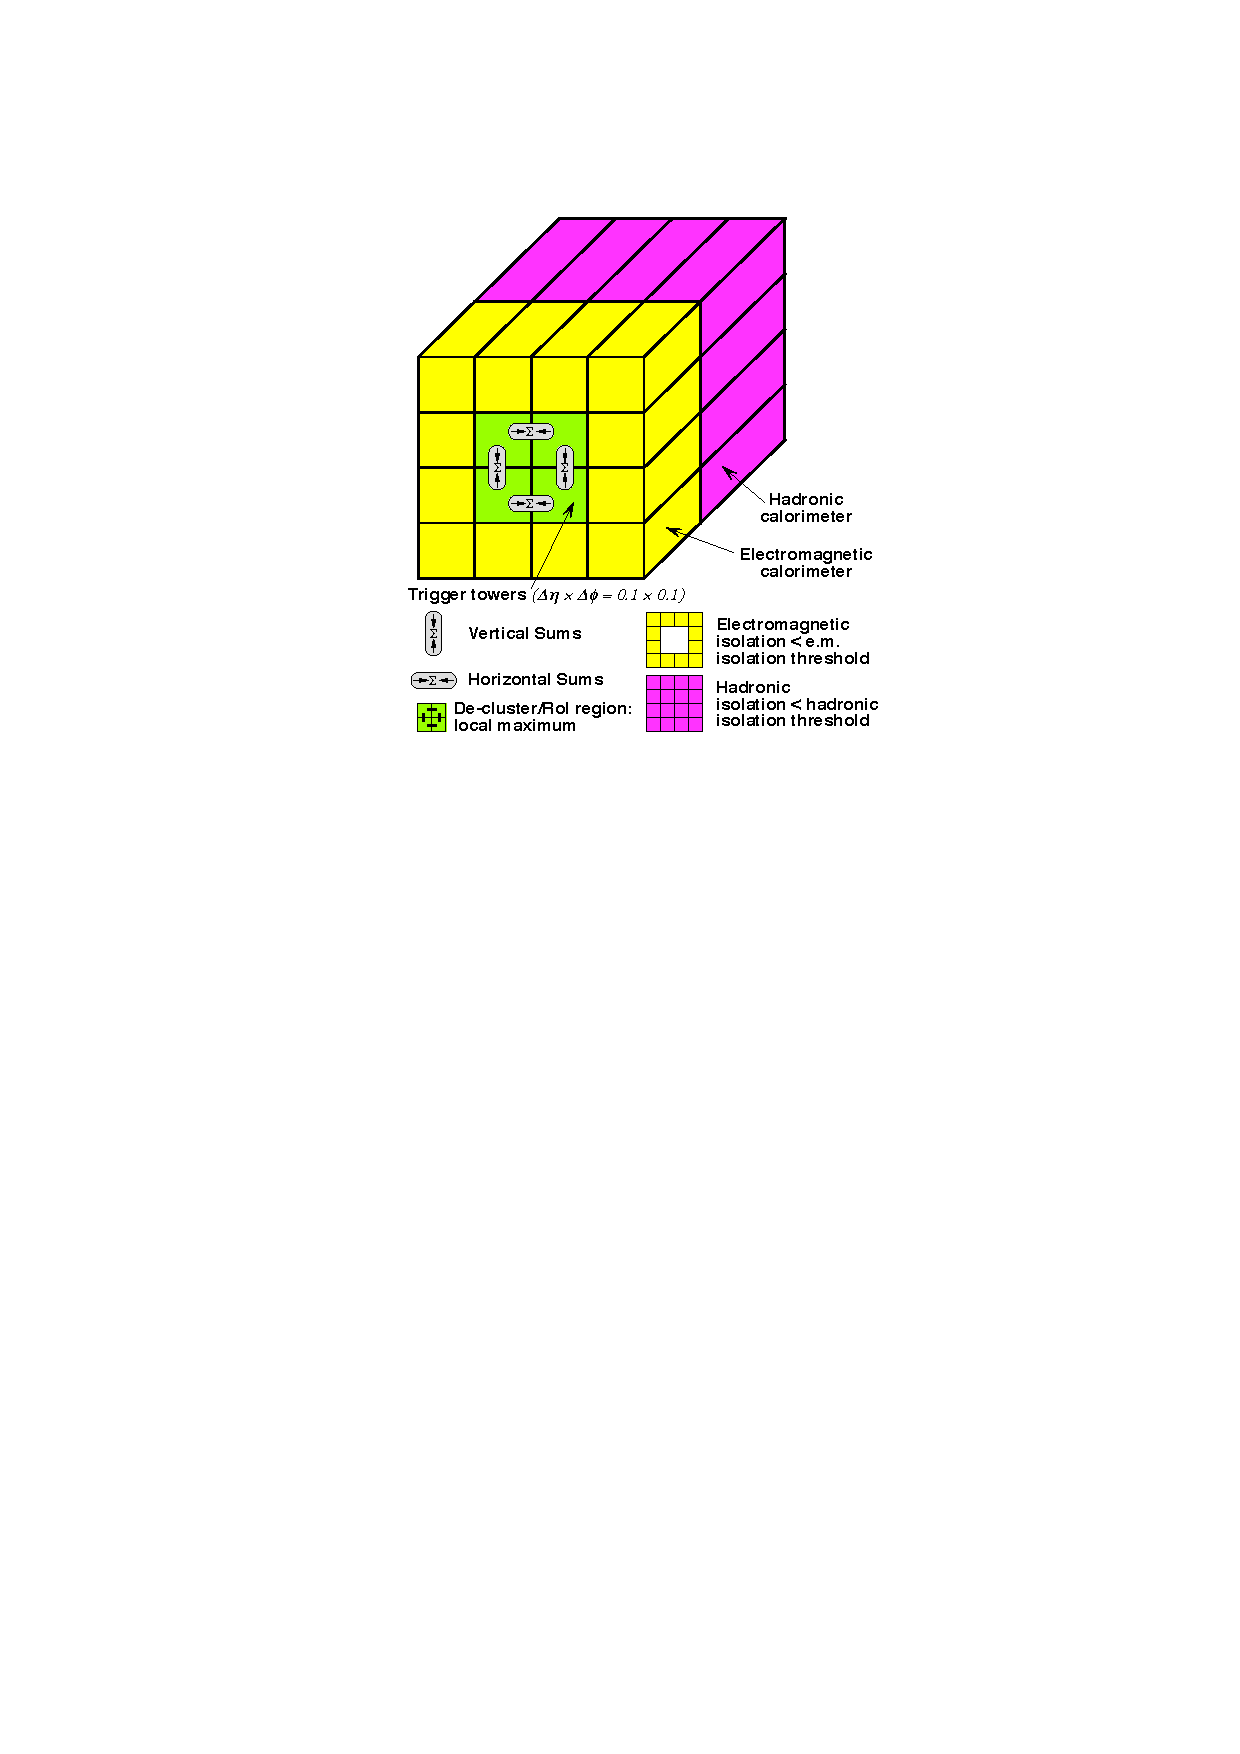
\includegraphics[width=0.4\textwidth]{figures/sliding_window_l1.pdf}
\caption[Torres de Trigger do primeiro nível de Trigger]{Torres de Trigger utilizadas para a seleção de elétrons no L1 do ATLAS. }
\label{fig:sliding_window_l1}
\end{figure}

\begin{itemize}
\item A soma das torres (EM e HAD) numa região $2\times2$ torres  em $\eta\times\phi$ localizadas no centro da janela de análise de L1: Esta hipótese é considerada bem sucedida caso o valor obtido com a soma das torres supere um determinado valor de corte.

\item $E_{T}$: quatro \textit{clusters}\footnote{um grupo de células que definem a região de interação da partícula com o calorímetro} eletromagnéticos sobrepostos, correspondendo a soma de duas torres. O \textit{cluster} mais energético deve ser maior ou igual a um determinado valor para o teste de hipótese ser bem sucedido. Este algoritmo determina a energia transversa da região analisada pelo L1.

\end{itemize}

O primeiro teste de hipótese serve apenas para determinar uma possível região de interesse (RoI). No caso de cortes sem isolamento, a região será aprovada somente se o segundo teste for bem sucedido. Para cortes com isolamento, a região de analise precisa ser aprovada por mais 4 testes de hipótese listados a seguir:

\begin{itemize}

\item $HAD_{Core}$ (Núcleo hadrônico): Soma das quatro torres do calorímetro hadrônico, posicionadas atrás dos \textit{clusters} eletromagnéticos.  Este teste será bem sucedido
caso esta soma seja menor ou igual a um dado patamar.

\item $EM_{Isol}$: Anel de isolamento eletromagnético, consistindo na soma da energia transversa das 12 torres eletromagnéticas posicionadas ao redor dos quatro 
\textit{clusters} eletromagnéticos. O teste é considerado aprovado caso o valor resultante da soma das 12 torres seja menor ou igual ao patamar de decisão estabelecido
para este corte.

\item $HAD_{Isol}$: Anel de isolamento hadrônico, correspondente à soma da energia transversa das 12 torres hadrônicas posicionadas ao redor do núcleo hadrônico.
O teste de hipotese será considerado aprovado caso o valor resultante da soma das 12 torres seja menor ou igual ao patamar de decisão estabelecido pelo corte.  

\end{itemize}

Dependendo da configuração requerida para o sistema de filtragem, os testes de hipótese acima serão aplicados sequencialmente. Caso seja aprovada,  a região de interesse do calorímetro será etiquetada e enviada para o sistema de filtragem de alto nível, onde novas extrações de características e algoritmos de hipótese mais sofisticados serão aplicados.

\subsection{Arquitetura do \textit{High Level Trigger}}

O sistema de \textit{Trigger} de alto nível recebe as regiões de interesse marcadas pelo nível 1 e realiza extrações de características e testes de hipóteses mais sofisticados, com granularidade
mais fina que seu nível anterior, para tomar a decisão de aceitação ou rejeição do evento. Neste nível, a latência é da ordem de milessegundos, o que possibilita a utilização de algoritmos mais
robustos e de maior custo computacional. Além das células do calorímetro, este nível utiliza a informação dos detectores de traço do ATLAS para compor a informação que será repassada para os testes de hipótese da configuração requerida para aceitação de um determinado padrão de evento na cadeia de \textit{Trigger}.

A arquitetura deste sistema foi implementada em software utilizando as linguagens C++, para compor o núcleo dos algoritmos, devido à necessidade de velocidade, e $python$
para a configuração e montagem da cadeia de execução do \textit{Trigger}, devido à sua simplicidade, fácil manutenção e adaptação.  Além disso, o atual sistema deve respeitar dois conceitos
bastante distintos que são utilizados em sequência para reduzir a taxa de eventos ao longo da cadeia de \textit{Trigger}.  Em outras palavras, este sistema é dividido em dois subsistemas: O sistema de \textit{Trigger} rápido (\textit{Fast}), o antigo L2, e o de alta precisão (\textit{Precision}), antigamente chamado de EF.  A Figura~\ref{fig:egammaChain} mostra o esquema de execução do \textit{Trigger} de alto nível para o canal $e/\gamma$. 

 
\begin{figure}[h!t]
\centering
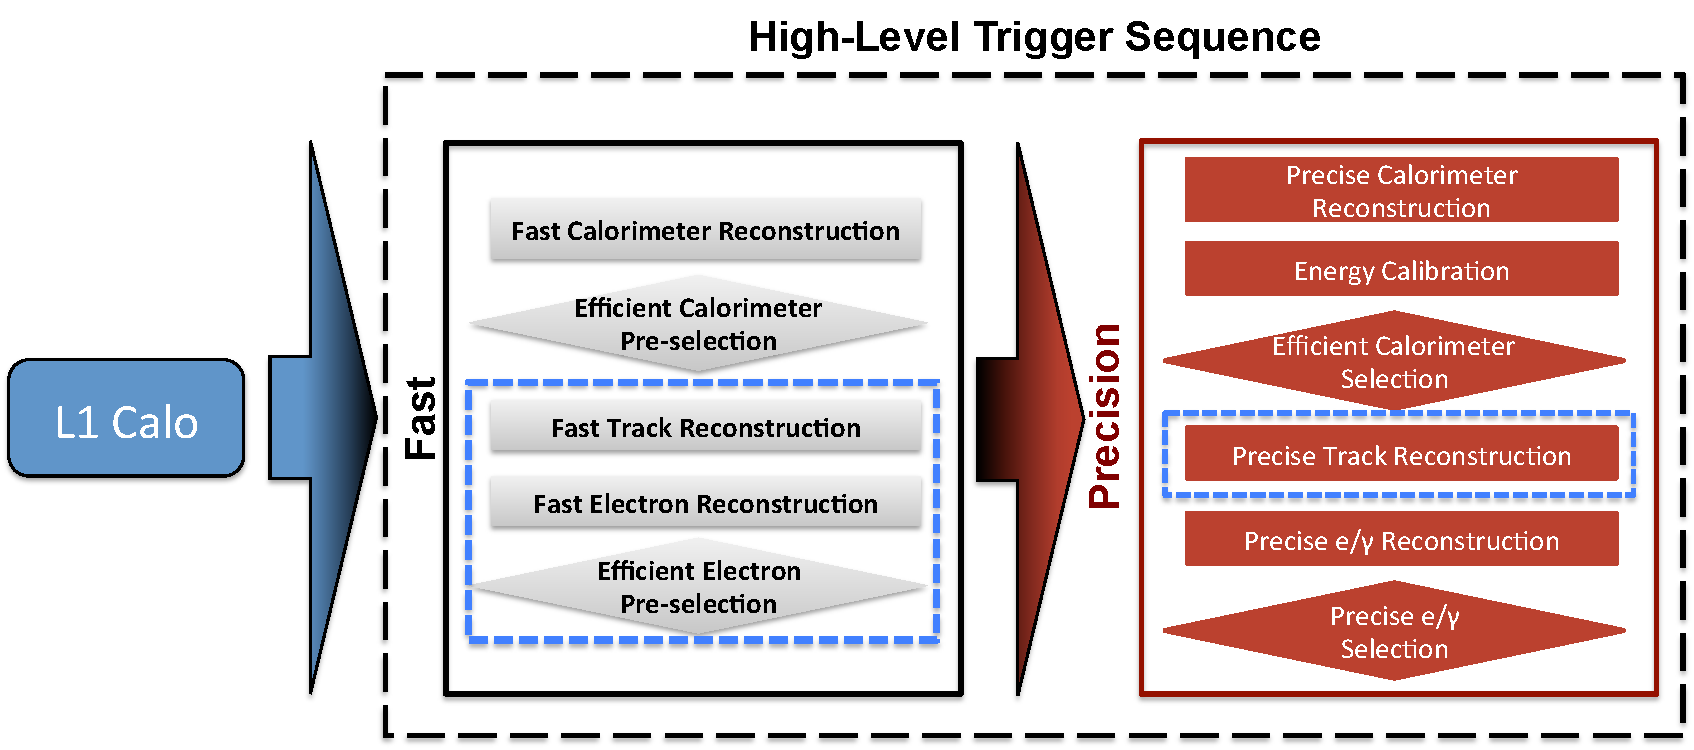
\includegraphics[width=0.8\textwidth]{figures/egammaChain.pdf}
\caption[Cadeia de execução dos algoritmos de \textit{trigger} do $e/\gamma$. ]
{Cadeia de execução dos algoritmos de extração de características (\textit{Reconstruction}), calibração e de testes de hipótese (\textit{Pre-selection} ou \textit{Selection}) para uma
configuração do $e/\gamma$. Extraído de \cite{artigo_acat2016_joao}.}
\label{fig:egammaChain}
\end{figure}

\subsubsection{Reconstrução Rápida do Calorímetro (\textit{Fast Calorimeter Reconstruction})}

Após receber a informação da RoI aceita pelo nível 1 com uma taxa de $\sim$100$k$Hz, o sistema de \textit{Trigger} rápido executa a reconstrução e extração de características do calorímetro com 
maior resolução utilizando um algoritmo para reconstrução de elétrons ou fótons baseado nas informações do chuveiro chamado de L2Calo. Esse, por sua vez, é uma versão limitada do algoritmo 
implementado na reconstrução precisa do calorímetro, devido à menor latência deste nível. A primeira etapa do L2Calo é refinar a posição em $\eta\times\phi$ da RoI, através do cálculo do 
baricentro da mesma, empregando, para tal, as células da segunda camada do calorímetro eletromagnético em sua granularidade mais fina. Em seguida, o L2Calo analisa
a energia e o perfil lateral e longitudinal do chuveiro produzido, resumindo esta informação em 4 variáveis. Estas variáveis são:

\begin{itemize}

\item Razão do Núcleo ($R_{core}$): Para a $2^{a}$ camada eletromagnética, $R_{core} = E_{3\times7}/E_{7\times7}$, onde $E_{m\times n}$ é a energia depositada em uma
região de $m\times n$ células em $\eta\times\phi$ ao redor da célula quente desta camada.

\item Razão de Energia ($E_{ratio}$): Para a $1^{a}$ camada eletromagnética, $E_{ratio} = (E_{1}-E_{2})/(E_{1}+E_{2})$, calculada em uma região de 
$\Delta\eta\times\Delta\phi = 0,125\times0,2$ ao redor do baricentro da RoI. $E_{1}$ e $E_{2}$ são, respectivamente, a primeira e a segunda célula
de maior energia.

\item Energia Transversa Eletromagnética ($E_{T_{EM}}$): É a energia transversa total depositada, nas 3 camadas eletromagnéticas, em uma região de 
$3\times7$ células em $\eta\times\phi$, centrada na célula quente da $2^{a}$ camada eletromagnética.
 
\item Razão de Energia Eletromagnética e Hadrônica ($E_{HAD}/E_{EM}$): $E_{HAD}$ é a energia transversa total depositada, nas 3 camadas hadrônicas, em 
uma janela de $\Delta\eta\times\Delta\phi=0, 2\times0, 2$ centrada no baricentro da RoI. 

\end{itemize}

\subsubsection{Seleção Eficiente do Calorímetro (\textit{Efficient Calorimeter Pre-selection})}

A próxima etapa da cadeia de \textit{Trigger} será aplicar o algoritmo de hipótese baseado nas variáveis de calorimetria extraídas da etapa de reconstrução rápida. O atual
algoritmo, chamado de T2Calo, realiza cortes lineares para cada uma das variáveis citadas anteriormente. Esses cortes são ajustados dependendo da assinatura requerida
pelo menu de \textit{Trigger} usado pela colaboração no momento da colisão ou simulação. O objetivo deste discriminador é reduzir a taxa de eventos utilizando somente
as células do calorímetro diminuindo assim o número de vezes que o algoritmo de traço, cujo custo computacional é mais alto, será executado na próxima etapa. 

\subsubsection{Reconstrução do traço e Pré-seleção de Elétrons (\textit{Fast Track Reconstruction and Efficient Electron Pre-selection})}

Nesta última etapa do \textit{Trigger} rápido os eventos aprovados pelo discriminador anterior executarão a reconstrução do traço utilizando o \gls{ftk}.
O \gls{ftk} é um sistema implementado em \gls{fpga} que recebe um conjunto de pontos do detector de  traço e, por meio de reconhecimento de padrão, retorna 
a trajetória da partícula caso, de fato, esses pontos definam uma trajetória.  Nessa etapa é computado o número de pontos ativados no detector de traço e o $p_{T}$. Então, o algoritmo de reconstrução de elétrons, chamado de L2Electron,  acessa essas informações e combina-as com as de calorimetria para usá-las na tomada de 
decisão na fase de teste de hipótese. Por fim, essa tomada de decisão é chamada de passo eficiente de pré-seleção de elétrons (\textit{Efficient Electron Pre-selection}).

\subsubsection{Reconstrução Precisa do Calorímetro, Calibração e Seleção Eficiente do Calorímetro}

Toda a infraestrutura que descreve o evento físico, no caso o objeto $e/\gamma$, na etapa precisa do \textit{Trigger} foi implementada de forma idêntica ao sistema de filtragem  \textit{offline}. 
Os algoritmos de reconstrução e os de hipóteses também foram idealizados de forma parecida porém de forma degradada devido aos requisitos de latência do sistema \textit{online}.  
Após receber os eventos aprovados no \textit{Trigger} na etapa anterior, a reconstrução do calorímetro é feita utilizando um algoritmo baseado nas informações do chuveiro da partícula
semelhante ao utilizado no L2Calo. No entanto,  esse possui uma maior complexidade e sofisticação na construção das variáveis devido aos algoritmos de ajuste e correções de energias
aplicados pela calibração nesta etapa, o que produz uma informação mais precisa e completa sobre a interação do evento com o calorímetro.

No teste de hipótese aplicado sobre os eventos desta etapa, pode-se escolher, atualmente, dois tipos de discriminadores configurados para atender a assinatura de  \textit{Trigger} requerida 
no momento da execução da cadeia de \textit{Trigger}. O primeiro deles é o T2Calo, que realiza os cortes lineares sobre as variareis extraídas do calorímetro. A outra opção é utilizar 
um \textit{Naive Bayes} como discriminador para tomar a decisão final nesta etapa de calorimetria, o que realiza os testes de hipótese por máxima verossimilhança (\textit{Likelihood, LH}).



\subsubsection{Reconstrução do Traço, do $e/\gamma$ e Seleção Precisa de Eventos}

No último estágio do \textit{Trigger}, a informação gerada na reconstrução do traço, utilizando um algoritmo mais complexo, combinada com a precisa informação de calorimetria gerada na etapa anterior 
é utilizada como entrada no teste final de hipótese. Com tudo, dependendo da configuração da assinatura aplicada na cadeia de \textit{Trigger}, um dos dois testes de hipótese
citados anteriormente pode ser utilizado para realizar essa discriminação. Por fim, combinando todos os testes de hipóteses aplicados no  \textit{Trigger} de alto nível, a taxa de eventos 
produzidos sofre uma redução dos $\sim$100$k$Hz iniciais após o primeiro nível de filtragem, para uma saída de aproximadamente 1$k$Hz, dependendo da assinatura de \textit{Trigger} requerida. 

\subsection{Sistema de Filtragem \textit{Offline}}

Conforme explicado no início deste capítulo, para sistemas de filtragem \textit{online}, uma vez que um evento é rejeitado, não é possível recuperar o mesmo. Desta forma,
para evitar a perda de um canal físico relevante, a eficiência de detecção é aumentada, com o custo de aumentar, também, o falso alarme. Consequentemente, ao final de um sistema
de filtragem \textit{online} ainda se encontram eventos, provenientes de ruído de fundo, misturados com os canais de interesse. Adicionalmente, os dados armazenados serão destinados
a inúmeros estudos distintos (bóson de Higgs, supersimetria, etc.), onde cada estudo necessitará observar um determinado subgrupo de eventos armazenados após a filtragem \textit{online}.

Para atender ao seu uso bastante diversificado, sistemas de filtragem \textit{offline} são empregados. Neste modelo de filtragem, uma vez que o tempo de processamento
não é um fator crítico, algoritmos mais complexos e eficientes podem ser empregados para analisar cada evento, de acordo com os requisitos específicos ao estudo sendo conduzido. Normalmente,
técnicas baseadas na estimação da função de densidade de probabilidade (PDF) do sinal de interesse são exploradas. Métodos \textit{bayesianos} de análise são frequentemente utilizados para testar
a hipótese de ocorrência de um determinado canal físico. Hipóteses também podem ser testadas ao comparar-se se a PDF do canal físico desejado está similar à distribuição de probabilidade
descrita pela teoria para este canal por meio de simulação de Monte Carlo. 

\subsection{Assinaturas de \textit{Trigger} e seus Sufixos}

Uma assinatura, também chamadas de \textit{chain}, é um esquema de configuração onde o nome do \textit{Trigger} é mapeado em uma lista de configurações e cortes realizados pelo sistema
de montagem do Trigger. A Tabela~\ref{tab:egammaChains_exemplos} mostra o esquema de configuração do primeiro nível de \textit{Trigger}, dos algoritmos de extração de 
características, do inglés \textit{Feature Extraction} (FEX), e de hipótese, \textit{Hypothesis} (HYPO)  para cada uma das \textit{chains}.  
Em geral, as \textit{chains} possuem critérios de ajustes na taxa de detecção e seleções especiais embutidos em seu próprio nome. Dentre os principais sufixos encontrados nos nomes das 
assinaturas podemos citar: 

\begin{itemize}

\item $e(E_{T_{cut}}$) ou $g(E_{T_{cut}}$): Representam assinaturas de elétrons ($e$) ou fótons ($g$) com $E_{T} > E_{T_{cut}} GeV$. Exemplo: e5, e25, g25, etc.

\item \textit{loose}, \textit{medium} e \textit{tight}: Esses sufixos representam ajustes nos cortes realizados pelos discriminadores aplicados na etapa de hipótese no \textit{Trigger} de alto nivel utilizando 
o T2Calo como base. Em geral, um critério \textit{loose} representa uma maior aceitação no \textit{Trigger} utilizando critérios mais relaxados. Em consequência disso, uma maior taxa de detecção e 
falso alarme são esperados para essa configuração. No entanto, para o critério \textit{tight} a ideia é oposta. Neste caso, uma amostra mais pura de eventos é extraída do \textit{Trigger} utilizando cortes mais 
apertados produzindo assim uma taxa de falso alarme bastante reduzida. Por fim, o critério \textit{medium} realiza o balanço entre esses dois casos.

\item \textit{lhloose}, \textit{lhmedium} e \textit{lhtight}: Representam a mesma ideia dos critérios acima porém utilizam a \textit{likelihood} como algoritmo de hipótese.

\item \textit{etcut}: O único corte aplicado nos algoritmos de hipótese é o de $E_{T}$ maior que um determinado valor em GeV;

\item \textit{iloose}: Exigência de evento isolado requerida para o \textit{Trigger}.

\end{itemize}

\begin{landscape}
% Please add the following required packages to your document preamble:
% \usepackage{multirow}
\begin{table}[p]\scriptsize
\centering
\begin{tabular}{ccccccccccc}
\hline
\hline
\multirow{4}{*}{\textit{\textbf{Chain}}} & \textbf{L1Calo} & \multicolumn{8}{c}{\textbf{HLT (\textit{High Level Trigger})}} & \multirow{4}{*}{\textbf{\begin{tabular}[c]{@{}c@{}}Ajuste \\ do corte\end{tabular}}} \\ \cline{3-10}
 &  & \multicolumn{4}{c}{\textit{\textbf{Fast}}} & \multicolumn{4}{c}{\textbf{Precision}} &  \\ \cline{3-10}
 &  & \multicolumn{2}{c}{\textbf{Calo}} & \multicolumn{2}{c}{\textbf{Electron}} & \multicolumn{2}{c}{\textbf{Calo}} & \multicolumn{2}{c}{\textbf{$e/\gamma$}} &  \\ \cline{3-10}
 &  & FEX & HYPO & FEX & HYPO & FEX & HYPO & FEX & HYPO &  \\ \hline
e24\_medium\_L1EM18VH & $E_{T} > 18GeV$ & Shower & T2Calo & \begin{tabular}[c]{@{}c@{}}FTK\\ +Shower\end{tabular} & \begin{tabular}[c]{@{}c@{}}T2Calo\\ Combined\end{tabular} & Shower & T2Calo & \begin{tabular}[c]{@{}c@{}}Shower\\ +Tracker\\ +Calibration\end{tabular} & \begin{tabular}[c]{@{}c@{}}T2Calo\\ Combined\end{tabular} & medium \\ \hline
e24\_lhmedium\_nod0\_iloose & \begin{tabular}[c]{@{}c@{}}$E_{T} > 20GeV$\\ Isolated\end{tabular} & Shower & T2Calo & \begin{tabular}[c]{@{}c@{}}FTK\\ +Shower\end{tabular} & \begin{tabular}[c]{@{}c@{}}T2Calo\\ Combined\end{tabular} & Shower & Likelihood & \begin{tabular}[c]{@{}c@{}}Shower\\ +Tracker\\ +Calibration\end{tabular} & \begin{tabular}[c]{@{}c@{}}Likelihood\\ Isolated\end{tabular} & medium \\ \hline
e24\_tight\_L1EM22VHI & \begin{tabular}[c]{@{}c@{}}$E_{T} > 22GeV$\\ Isolated\end{tabular} & Shower & T2Calo & \begin{tabular}[c]{@{}c@{}}FTK\\ +Shower\end{tabular} & \begin{tabular}[c]{@{}c@{}}T2Calo\\ Combined\end{tabular} & Shower & T2Calo & \begin{tabular}[c]{@{}c@{}}Shower\\ +Tracker\\ +Calibration\end{tabular} & T2Calo & tight \\ \hline
e5\_etcut & $E_{T} > 3GeV$ & Shower & No Cut & \begin{tabular}[c]{@{}c@{}}FTK\\ +Shower\end{tabular} & No Cut & Shower & $E_{T}$ \textgreater 5GeV & \begin{tabular}[c]{@{}c@{}}Shower\\ +Tracker\\ +Calibration\end{tabular} & No Cut &  \\ \hline \hline
\end{tabular}
\centering

\caption[Descrição de algumas assinaturas aplicadas no \textit{Trigger}]
{Descrição das configurações de \textit{Trigger} para cada uma das  \textit{chains}.  Os cortes em energia para o nível 1 estão representados na coluna 
do L1Calo. Cada posição do HLT foi preenchida com o nome do respectivo algoritmo para sua \gls{fex} e \gls{hypo} respectivamente. }

\label{tab:egammaChains_exemplos}
\end{table}

\end{landscape}


